% Options for packages loaded elsewhere
\PassOptionsToPackage{unicode}{hyperref}
\PassOptionsToPackage{hyphens}{url}
%
\documentclass[
  oneside,
  open=any]{scrbook}

\usepackage{amsmath,amssymb}
\usepackage{iftex}
\ifPDFTeX
  \usepackage[T1]{fontenc}
  \usepackage[utf8]{inputenc}
  \usepackage{textcomp} % provide euro and other symbols
\else % if luatex or xetex
  \usepackage{unicode-math}
  \defaultfontfeatures{Scale=MatchLowercase}
  \defaultfontfeatures[\rmfamily]{Ligatures=TeX,Scale=1}
\fi
\usepackage{lmodern}
\ifPDFTeX\else  
    % xetex/luatex font selection
\fi
% Use upquote if available, for straight quotes in verbatim environments
\IfFileExists{upquote.sty}{\usepackage{upquote}}{}
\IfFileExists{microtype.sty}{% use microtype if available
  \usepackage[]{microtype}
  \UseMicrotypeSet[protrusion]{basicmath} % disable protrusion for tt fonts
}{}
\makeatletter
\@ifundefined{KOMAClassName}{% if non-KOMA class
  \IfFileExists{parskip.sty}{%
    \usepackage{parskip}
  }{% else
    \setlength{\parindent}{0pt}
    \setlength{\parskip}{6pt plus 2pt minus 1pt}}
}{% if KOMA class
  \KOMAoptions{parskip=half}}
\makeatother
\usepackage{xcolor}
\setlength{\emergencystretch}{3em} % prevent overfull lines
\setcounter{secnumdepth}{5}
% Make \paragraph and \subparagraph free-standing
\ifx\paragraph\undefined\else
  \let\oldparagraph\paragraph
  \renewcommand{\paragraph}[1]{\oldparagraph{#1}\mbox{}}
\fi
\ifx\subparagraph\undefined\else
  \let\oldsubparagraph\subparagraph
  \renewcommand{\subparagraph}[1]{\oldsubparagraph{#1}\mbox{}}
\fi
\usepackage{color}
\usepackage{fancyvrb}
\newcommand{\VerbBar}{|}
\newcommand{\VERB}{\Verb[commandchars=\\\{\}]}
\DefineVerbatimEnvironment{Highlighting}{Verbatim}{commandchars=\\\{\}}
% Add ',fontsize=\small' for more characters per line
\usepackage{framed}
\definecolor{shadecolor}{RGB}{241,243,245}
\newenvironment{Shaded}{\begin{snugshade}}{\end{snugshade}}
\newcommand{\AlertTok}[1]{\textcolor[rgb]{0.68,0.00,0.00}{#1}}
\newcommand{\AnnotationTok}[1]{\textcolor[rgb]{0.37,0.37,0.37}{#1}}
\newcommand{\AttributeTok}[1]{\textcolor[rgb]{0.40,0.45,0.13}{#1}}
\newcommand{\BaseNTok}[1]{\textcolor[rgb]{0.68,0.00,0.00}{#1}}
\newcommand{\BuiltInTok}[1]{\textcolor[rgb]{0.00,0.23,0.31}{#1}}
\newcommand{\CharTok}[1]{\textcolor[rgb]{0.13,0.47,0.30}{#1}}
\newcommand{\CommentTok}[1]{\textcolor[rgb]{0.37,0.37,0.37}{#1}}
\newcommand{\CommentVarTok}[1]{\textcolor[rgb]{0.37,0.37,0.37}{\textit{#1}}}
\newcommand{\ConstantTok}[1]{\textcolor[rgb]{0.56,0.35,0.01}{#1}}
\newcommand{\ControlFlowTok}[1]{\textcolor[rgb]{0.00,0.23,0.31}{#1}}
\newcommand{\DataTypeTok}[1]{\textcolor[rgb]{0.68,0.00,0.00}{#1}}
\newcommand{\DecValTok}[1]{\textcolor[rgb]{0.68,0.00,0.00}{#1}}
\newcommand{\DocumentationTok}[1]{\textcolor[rgb]{0.37,0.37,0.37}{\textit{#1}}}
\newcommand{\ErrorTok}[1]{\textcolor[rgb]{0.68,0.00,0.00}{#1}}
\newcommand{\ExtensionTok}[1]{\textcolor[rgb]{0.00,0.23,0.31}{#1}}
\newcommand{\FloatTok}[1]{\textcolor[rgb]{0.68,0.00,0.00}{#1}}
\newcommand{\FunctionTok}[1]{\textcolor[rgb]{0.28,0.35,0.67}{#1}}
\newcommand{\ImportTok}[1]{\textcolor[rgb]{0.00,0.46,0.62}{#1}}
\newcommand{\InformationTok}[1]{\textcolor[rgb]{0.37,0.37,0.37}{#1}}
\newcommand{\KeywordTok}[1]{\textcolor[rgb]{0.00,0.23,0.31}{#1}}
\newcommand{\NormalTok}[1]{\textcolor[rgb]{0.00,0.23,0.31}{#1}}
\newcommand{\OperatorTok}[1]{\textcolor[rgb]{0.37,0.37,0.37}{#1}}
\newcommand{\OtherTok}[1]{\textcolor[rgb]{0.00,0.23,0.31}{#1}}
\newcommand{\PreprocessorTok}[1]{\textcolor[rgb]{0.68,0.00,0.00}{#1}}
\newcommand{\RegionMarkerTok}[1]{\textcolor[rgb]{0.00,0.23,0.31}{#1}}
\newcommand{\SpecialCharTok}[1]{\textcolor[rgb]{0.37,0.37,0.37}{#1}}
\newcommand{\SpecialStringTok}[1]{\textcolor[rgb]{0.13,0.47,0.30}{#1}}
\newcommand{\StringTok}[1]{\textcolor[rgb]{0.13,0.47,0.30}{#1}}
\newcommand{\VariableTok}[1]{\textcolor[rgb]{0.07,0.07,0.07}{#1}}
\newcommand{\VerbatimStringTok}[1]{\textcolor[rgb]{0.13,0.47,0.30}{#1}}
\newcommand{\WarningTok}[1]{\textcolor[rgb]{0.37,0.37,0.37}{\textit{#1}}}

\providecommand{\tightlist}{%
  \setlength{\itemsep}{0pt}\setlength{\parskip}{0pt}}\usepackage{longtable,booktabs,array}
\usepackage{calc} % for calculating minipage widths
% Correct order of tables after \paragraph or \subparagraph
\usepackage{etoolbox}
\makeatletter
\patchcmd\longtable{\par}{\if@noskipsec\mbox{}\fi\par}{}{}
\makeatother
% Allow footnotes in longtable head/foot
\IfFileExists{footnotehyper.sty}{\usepackage{footnotehyper}}{\usepackage{footnote}}
\makesavenoteenv{longtable}
\usepackage{graphicx}
\makeatletter
\def\maxwidth{\ifdim\Gin@nat@width>\linewidth\linewidth\else\Gin@nat@width\fi}
\def\maxheight{\ifdim\Gin@nat@height>\textheight\textheight\else\Gin@nat@height\fi}
\makeatother
% Scale images if necessary, so that they will not overflow the page
% margins by default, and it is still possible to overwrite the defaults
% using explicit options in \includegraphics[width, height, ...]{}
\setkeys{Gin}{width=\maxwidth,height=\maxheight,keepaspectratio}
% Set default figure placement to htbp
\makeatletter
\def\fps@figure{htbp}
\makeatother
% definitions for citeproc citations
\NewDocumentCommand\citeproctext{}{}
\NewDocumentCommand\citeproc{mm}{%
  \begingroup\def\citeproctext{#2}\cite{#1}\endgroup}
\makeatletter
 % allow citations to break across lines
 \let\@cite@ofmt\@firstofone
 % avoid brackets around text for \cite:
 \def\@biblabel#1{}
 \def\@cite#1#2{{#1\if@tempswa , #2\fi}}
\makeatother
\newlength{\cslhangindent}
\setlength{\cslhangindent}{1.5em}
\newlength{\csllabelwidth}
\setlength{\csllabelwidth}{3em}
\newenvironment{CSLReferences}[2] % #1 hanging-indent, #2 entry-spacing
 {\begin{list}{}{%
  \setlength{\itemindent}{0pt}
  \setlength{\leftmargin}{0pt}
  \setlength{\parsep}{0pt}
  % turn on hanging indent if param 1 is 1
  \ifodd #1
   \setlength{\leftmargin}{\cslhangindent}
   \setlength{\itemindent}{-1\cslhangindent}
  \fi
  % set entry spacing
  \setlength{\itemsep}{#2\baselineskip}}}
 {\end{list}}
\usepackage{calc}
\newcommand{\CSLBlock}[1]{\hfill\break\parbox[t]{\linewidth}{\strut\ignorespaces#1\strut}}
\newcommand{\CSLLeftMargin}[1]{\parbox[t]{\csllabelwidth}{\strut#1\strut}}
\newcommand{\CSLRightInline}[1]{\parbox[t]{\linewidth - \csllabelwidth}{\strut#1\strut}}
\newcommand{\CSLIndent}[1]{\hspace{\cslhangindent}#1}

\usepackage{tabularx, lipsum}
\usepackage{color,soul}
\makeatletter
\@ifpackageloaded{caption}{}{\usepackage{caption}}
\AtBeginDocument{%
\ifdefined\contentsname
  \renewcommand*\contentsname{Table of contents}
\else
  \newcommand\contentsname{Table of contents}
\fi
\ifdefined\listfigurename
  \renewcommand*\listfigurename{List of Figures}
\else
  \newcommand\listfigurename{List of Figures}
\fi
\ifdefined\listtablename
  \renewcommand*\listtablename{List of Tables}
\else
  \newcommand\listtablename{List of Tables}
\fi
\ifdefined\figurename
  \renewcommand*\figurename{Figure}
\else
  \newcommand\figurename{Figure}
\fi
\ifdefined\tablename
  \renewcommand*\tablename{Table}
\else
  \newcommand\tablename{Table}
\fi
}
\@ifpackageloaded{float}{}{\usepackage{float}}
\floatstyle{ruled}
\@ifundefined{c@chapter}{\newfloat{codelisting}{h}{lop}}{\newfloat{codelisting}{h}{lop}[chapter]}
\floatname{codelisting}{Listing}
\newcommand*\listoflistings{\listof{codelisting}{List of Listings}}
\makeatother
\makeatletter
\makeatother
\makeatletter
\@ifpackageloaded{caption}{}{\usepackage{caption}}
\@ifpackageloaded{subcaption}{}{\usepackage{subcaption}}
\makeatother

\usepackage{hyphenat}
\usepackage{ifthen}
\usepackage{calc}
\usepackage{calculator}

\usepackage{graphicx}
\usepackage{wallpaper}

\usepackage{geometry}

\usepackage{graphicx}
\usepackage{geometry}
\usepackage{afterpage}
\usepackage{tikz}
\usetikzlibrary{calc}
\usetikzlibrary{fadings}
\usepackage[pagecolor=none]{pagecolor}


% Set the titlepage font families







% Set the coverpage font families

\ifLuaTeX
  \usepackage{selnolig}  % disable illegal ligatures
\fi
\usepackage{bookmark}

\IfFileExists{xurl.sty}{\usepackage{xurl}}{} % add URL line breaks if available
\urlstyle{same} % disable monospaced font for URLs
\hypersetup{
  pdftitle={Cataloguing and visualizing big Geodata},
  pdfauthor={Martín Domínguez Durán},
  hidelinks,
  pdfcreator={LaTeX via pandoc}}

\title{Cataloguing and visualizing big Geodata}
\usepackage{etoolbox}
\makeatletter
\providecommand{\subtitle}[1]{% add subtitle to \maketitle
  \apptocmd{\@title}{\par {\large #1 \par}}{}{}
}
\makeatother
\subtitle{Final report}
\author{Martín Domínguez Durán}
\date{}

\begin{document}
%%%%% begin titlepage extension code

  \begin{frontmatter}

\begin{titlepage}

%%% TITLE PAGE START

% Set up alignment commands
%Page
\newcommand{\titlepagepagealign}{
\ifthenelse{\equal{left}{right}}{\raggedleft}{}
\ifthenelse{\equal{left}{center}}{\centering}{}
\ifthenelse{\equal{left}{left}}{\raggedright}{}
}


\newcommand{\titleandsubtitle}{
% Title and subtitle
{{\large{\bfseries{\nohyphens{Cataloguing and visualizing big
Geodata}}}}\par
}%

\vspace{\betweentitlesubtitle}
{
{\large{\textit{\nohyphens{Final report}}}}\par
}}
\newcommand{\titlepagetitleblock}{
\titleandsubtitle
}

\newcommand{\authorstyle}[1]{{\large{#1}}}

\newcommand{\affiliationstyle}[1]{{\large{#1}}}

\newcommand{\titlepageauthorblock}{
{\authorstyle{\nohyphens{Martín Domínguez Durán}{\textsuperscript{1}}}}}

\newcommand{\titlepageaffiliationblock}{
\hangindent=1em
\hangafter=1
{\affiliationstyle{
{1}.~Wageningen University \& Research,~Wageningen, The Netherlands


\vspace{1\baselineskip} 
}}
}
\newcommand{\headerstyled}{%
{The Publisher}
}
\newcommand{\footerstyled}{%
{\large{\textbf{Registration number:} 1254246\\
\textbf{Period of Internship:} 2024-04-08 - 2024-08-08\\
\textbf{Date final report:} 2024-07-31\\
\textbf{Telephone number student:} +31651120353\\
\textbf{Name of Company:} Satelligence B.V.\\
\textbf{Host supervisor:} Luca Foresta\\
\textbf{MGI supervisor:} Lukasz Grus}}
}
\newcommand{\datestyled}{%
{}
}


\newcommand{\titlepageheaderblock}{\headerstyled}

\newcommand{\titlepagefooterblock}{
\footerstyled
}

\newcommand{\titlepagedateblock}{
\datestyled
}

%set up blocks so user can specify order
\newcommand{\titleblock}{\newlength{\betweentitlesubtitle}
\setlength{\betweentitlesubtitle}{\baselineskip}
{

{\titlepagetitleblock}
}

\vspace{4\baselineskip}
}

\newcommand{\authorblock}{{\titlepageauthorblock}

\vspace{2\baselineskip}
}

\newcommand{\affiliationblock}{{\titlepageaffiliationblock}

\vspace{1pt}
}

\newcommand{\logoblock}{{
\includegraphics[width=0.7\textheight]{img/logo.png}}

\vspace{2\baselineskip}
}

\newcommand{\footerblock}{{\titlepagefooterblock}

\vspace{1pt}
}

\newcommand{\dateblock}{}

\newcommand{\headerblock}{{\titlepageheaderblock

\vspace{0pt}
}}
\newgeometry{top=3in,bottom=1in,right=1in,left=1in}
% background image
\newlength{\bgimagesize}
\setlength{\bgimagesize}{0.5\paperwidth}
\LENGTHDIVIDE{\bgimagesize}{\paperwidth}{\theRatio} % from calculator pkg
\ThisULCornerWallPaper{\theRatio}{img/corner-bg.png}

\thispagestyle{empty} % no page numbers on titlepages


\newcommand{\vrulecode}{\rule{\vrulewidth}{\textheight}}
\newlength{\vrulewidth}
\setlength{\vrulewidth}{1pt}
\newlength{\B}
\setlength{\B}{\ifdim\vrulewidth > 0pt 0.05\textwidth\else 0pt\fi}
\newlength{\minipagewidth}
\ifthenelse{\equal{left}{left} \OR \equal{left}{right} }
{% True case
\setlength{\minipagewidth}{\textwidth - \vrulewidth - \B - 0.1\textwidth}
}{
\setlength{\minipagewidth}{\textwidth - 2\vrulewidth - 2\B - 0.1\textwidth}
}
\ifthenelse{\equal{left}{left} \OR \equal{left}{leftright}}
{% True case
\raggedleft % needed for the minipage to work
\vrulecode
\hspace{\B}
}{%
\raggedright % else it is right only and width is not 0
}
% [position of box][box height][inner position]{width}
% [s] means stretch out vertically; assuming there is a vfill
\begin{minipage}[b][\textheight][s]{\minipagewidth}
\titlepagepagealign
\titleblock

\authorblock

\affiliationblock

\vfill

\logoblock

\footerblock
\par

\end{minipage}\ifthenelse{\equal{left}{right} \OR \equal{left}{leftright} }{
\hspace{\B}
\vrulecode}{}
\clearpage
\restoregeometry
%%% TITLE PAGE END
\end{titlepage}
\setcounter{page}{1}
\end{frontmatter}

%%%%% end titlepage extension code

\renewcommand*\contentsname{Table of contents}
{
\setcounter{tocdepth}{2}
\tableofcontents
}
\listoffigures
\mainmatter
\chapter*{Executive summary}\label{executive-summary}
\addcontentsline{toc}{chapter}{Executive summary}

\lipsum

\newpage

\chapter*{List of abreviations}\label{list-of-abreviations}
\addcontentsline{toc}{chapter}{List of abreviations}

\begin{longtable}[]{@{}
  >{\raggedright\arraybackslash}p{(\columnwidth - 2\tabcolsep) * \real{0.5556}}
  >{\raggedright\arraybackslash}p{(\columnwidth - 2\tabcolsep) * \real{0.4444}}@{}}
\caption{Abbreviation list}\tabularnewline
\toprule\noalign{}
\begin{minipage}[b]{\linewidth}\raggedright
\textbf{Abreviations}
\end{minipage} & \begin{minipage}[b]{\linewidth}\raggedright
\textbf{Description}
\end{minipage} \\
\midrule\noalign{}
\endfirsthead
\toprule\noalign{}
\begin{minipage}[b]{\linewidth}\raggedright
\textbf{Abreviations}
\end{minipage} & \begin{minipage}[b]{\linewidth}\raggedright
\textbf{Description}
\end{minipage} \\
\midrule\noalign{}
\endhead
\bottomrule\noalign{}
\endlastfoot
EUDR & European Union Deforestation Regulation \\
STAC & Spatio-Temporal Asset Catalog \\
COG & Cloud-Optimized GeoTiff \\
OGC & Open Geospatial Consortium \\
SDI & Spatial Data Infrastructure \\
S11 & Satelligence \\
K8 & Kubernetes \\
DPROF & Distributed Processing Framework \\
JSON & JavaScript Object Notation \\
API & Application Programming Interfaces \\
HTTP & HyperText Transfer Protocol \\
SQL & Standard Query Language \\
\end{longtable}

\chapter{Introduction}\label{introduction}

\section{Internship organization
background}\label{internship-organization-background}

Satelligence (S11) is a company founded in 2016 that specializes in
providing satellite-based actionable information by monitoring
environmental risks in commodity supply chains and financial investment
planning (\citeproc{ref-satelligence_home_nodate}{Satelligence, n.d.}).
More specifically, the company processes terabytes of satellite imagery
to detect environmental risks and presents this information to their
clients in a web application to assist them in the migration towards
more sustainable sourcing models and the compliance with
deforestation-free commodities regulations, such as the European Union
Deforestation Regulation (EUDR)
(\citeproc{ref-satelligence_internship_2023}{Satelligence, 2023}). S11's
main focus is continuous deforestation monitoring (CDM) in the tropics
using freely accessible satellite imagery. This is a data-intensive task
that is achieved by leveraging the benefits of cloud computing,
specifically Google Cloud Platform.

\section{Context and justification of
research}\label{context-and-justification-of-research}

Satelligence strongly relies on cloud computing for their services. They
process extensive volumes of satellite imagery amounting to terabytes
using DPROF, a distributed processing framework created within the
company to efficiently process multidimensional spatial datasets. While
this processing workflow currently runs smoothly, the company's data and
operations teams face challenges when going deeper into the analysis and
accessing intermediate results due to the big nature of this data
(\citeproc{ref-satelligence_internship_2023}{Satelligence, 2023}).
Scholars have defined big data as datasets characterized by their high
Volume, Velocity, and Variety, which makes it paramount to use advanced
processing and analytics techniques to derive relevant insights
(\citeproc{ref-giri_big_2014}{Giri and Lone, 2014}). In the specific
case of Satelligence, their datasets can be categorized as big data due
to their: High volume (Terabytes of satellite images processed every
day), high velocity (Near -- real time processing of these images) and
high variety (Imagery coming from different sensors and regions). All
these datasets are a specific case of big data: Big Geodata.

\subsection{Significance of the topic and previous
research}\label{significance-of-the-topic-and-previous-research}

In the past decades there has been a rapid increase in the amount and
size of geo-spatial information that can be accessed. Nowadays, more
than 150 satellites orbit the earth collecting thousands of images every
single day (\citeproc{ref-zhao_scalable_2021}{Zhao et al., 2021}). This
has made data handling and the introduction of spatial data
infrastructures (SDIs) paramount when working with such big datasets.

Traditionally, SDIs have served to ease the accessibility, integration
and analysis of spatial data
(\citeproc{ref-rajabifard_spatial_2001}{Rajabifard and Williamson,
2001}). However, in practice SDIs have been built upon technologies that
focus on data preservation rather than accessibility
(\citeproc{ref-durbha_advances_2023}{Durbha et al., 2023}). Due to this,
an important shift is underway towards more cloud-based SDIs
(\citeproc{ref-tripathi_cloud_2020}{Tripathi et al., 2020}). These
platforms need the emergence of new technologies that prioritize
seamless access to cloud-stored data, efficient discovery services that
ensure the easy location of extensive spatial data, and data
visualization interfaces where multiple datasets can be depicted.

\subsubsection*{Cloud-based data
storage}\label{cloud-based-data-storage}
\addcontentsline{toc}{subsubsection}{Cloud-based data storage}

Spatial data, just like any other type of data, can be cataloged into
structured and unstructured data. Structured datasets are often
organized and follow a specific structure (i.e.~A traditional table with
rows (objects) and columns (features)). On the other hand, unstructured
data does not have a predefined structure (e.g.~Satellite imagery and
Time series data) (\citeproc{ref-mishra_structured_2017}{Mishra and
Misra, 2017}). The management of structured data has witnessed
substantial advancements, making it straightforward to handle it
systematically using, for instance, relational databases (i.e.~With the
help of Structured Query Language (SQL))
(\citeproc{ref-kaufmann_database_2023}{Kaufmann and Meier, 2023}). In
contrast, due to the additional challenges associated with the handling
of unstructured data, the developments in this area have taken a longer
time to appear.

The emergence of cloud-based archives has been one of the main
advancements for unstructured data management during the last decades.
In the specific case of geo-spatial data, it has allowed to store
terabytes of unstructured data (i.e.~Satellite imagery) on the cloud and
access it through the network. However, the necessity transmitting data
across networks to access it makes it essential to develop new data
formats suited for such purposes
(\citeproc{ref-durbha_advances_2023}{Durbha et al., 2023}).

At S11, the storage of large geo-spatial data is already managed using
Google Storage Buckets, and they are currently in the process of
incorporating the conversion to cloud-optimized data formats like Cloud
Optimized GeoTIFFs (COGs) and Zarrs in their processing framework
(DPROF) to improve efficiency and accessibility.

\paragraph*{Cloud-optimized data
formats}\label{cloud-optimized-data-formats}
\addcontentsline{toc}{paragraph}{Cloud-optimized data formats}

\subparagraph*{COG}\label{cog}
\addcontentsline{toc}{subparagraph}{COG}

Cloud-Optimized GeoTIFFs (\href{https://www.cogeo.org/}{COGs}) are an
example of data formats that have been created to ease the access of
data stored in the cloud. They improve the readability by including the
metadata in the initial bytes of the file stored, storing different
image overviews for different scales and tiling the images in smaller
blocks. These characteristics make COG files heavier than traditional
image formats. However, they also greatly enhance accessibility by
enabling the selective transfer of only the necessary tiles using HTTP
GET requests (\citeproc{ref-desruisseaux_ogc_2021}{Desruisseaux et al.,
2021}). Additionally, this data format has been adopted as an Open
Geospatial Consortium (OGC) standard. These standards are a set of
guidelines and specifications created to facilitat data interoperability
(\citeproc{ref-ogc_ogc_2023}{OGC, 2023}).

\subparagraph*{Zarr}\label{zarr}
\addcontentsline{toc}{subparagraph}{Zarr}

Another cloud native data format that has gained popularity recently is
\href{https://zarr.readthedocs.io/en/stable/}{Zarr}. This data format
and python library focuses on the cloud-optimization of n-dimensional
arrays. Zarr, differently than COGs store the metadata separately from
the data chunks using lightweight external JSON files
(\citeproc{ref-durbha_advances_2023}{Durbha et al., 2023}).
Additionally, this data format stores the N-dimensional arrays in
smaller chunks that can be accessed more easily. While the storage of
Zarr files in chunks facilitates more efficient data access, the absence
of overviews hinders the visualization of this data in a web map service
(\citeproc{ref-desruisseaux_ogc_2021}{Desruisseaux et al., 2021}). Due
to the increasing use of Zarr for geo-spatial purposes, the OGC endorsed
Zarr V2 as a community standard. Nevertheless, efforts are still being
made to have a geo-spatial Zarr standard adopted by OGC
(\citeproc{ref-chester_ogc_2024}{Chester, 2024}).

\subsubsection*{Data discovery services}\label{data-discovery-services}
\addcontentsline{toc}{subsubsection}{Data discovery services}

A discovery service that recently has become widely used for the
exploration of big geo-data is Spatio-Temporal Asset Catalog (STAC).
Through the standardization of spatio-temporal metadata, STAC simplifies
the management and discovery of big geo-data
(\citeproc{ref-brodeur_geographic_2019}{Brodeur et al., 2019}). This
service works by organizing the data into catalogs, collections, items,
and assets stored as lightweight JSON formats (See
Table~\ref{tbl-stac-comps}) (\citeproc{ref-durbha_advances_2023}{Durbha
et al., 2023}).

Moreover, there are two types of STAC catalogs: static and dynamic.
Static catalogs are pre-generated and stored as static JSON files on a
cloud storage. Static catalogs follow sensible hierarchical
relationships between STAC components and this feature makes it easy to
be browsed and/or crawled by. Nevertheless, these catalogs cannot be
queried. On the other hand, dynamic catalogs are generated as APIs that
respond to queries dynamically. Notably, dynamic catalogs will show
different views of the same catalog depending on queries which usually
focus on the spatio-temporal aspect of the data
(\citeproc{ref-noauthor_stac-specbest-practicesmd_nodate}{RadiantEarth,
2024}).

\begin{longtable}[]{@{}
  >{\raggedright\arraybackslash}p{(\columnwidth - 2\tabcolsep) * \real{0.5556}}
  >{\raggedright\arraybackslash}p{(\columnwidth - 2\tabcolsep) * \real{0.4444}}@{}}
\caption{STAC components}\label{tbl-stac-comps}\tabularnewline
\toprule\noalign{}
\begin{minipage}[b]{\linewidth}\raggedright
\textbf{STAC components}
\end{minipage} & \begin{minipage}[b]{\linewidth}\raggedright
\textbf{Description}
\end{minipage} \\
\midrule\noalign{}
\endfirsthead
\toprule\noalign{}
\begin{minipage}[b]{\linewidth}\raggedright
\textbf{STAC components}
\end{minipage} & \begin{minipage}[b]{\linewidth}\raggedright
\textbf{Description}
\end{minipage} \\
\midrule\noalign{}
\endhead
\bottomrule\noalign{}
\endlastfoot
\emph{Assets} & An asset can be any type of data with a spatial and a
temporal component. \\
\emph{Items} & An item is a GeoJSON feature with some specifications
like: Time, Link to the asset (e.g.~Google bucket) \\
\emph{Collections} & Defines a set of common fields to describe a group
of Items that share properties and metadata \\
\emph{Catalogs} & Contains a list of STAC collections, items or can also
contain child catalogs. \\
\end{longtable}

In the specific case of dynamic catalogs, the concept of
\href{https://github.com/radiantearth/stac-api-spec/}{STAC API} is
widely used. In general, an API is a set of rules and protocols that
enables different software applications to communicate with each other.
In the case of the STAC API, it provides endpoints for searching and
retrieving geospatial data based on criteria such as location and time,
delivering results in a standardized format that ensures compatibility
with various tools and services in the geospatial community. Moreover,
even though STAC API is not an OGC standard or a OGC community standard,
the basic requests performed in a STAC API adheres to the
\href{https://ogcapi.ogc.org/features/}{OGC API-Features} standards for
querying by bounding box and time range, returning GeoJSON-formatted
results that conform to both STAC and OGC specifications. Ultimately,
compared to \href{https://ogcapi.ogc.org/features/}{OGC API-Features},
\href{https://github.com/radiantearth/stac-api-spec/}{STAC API} enhances
functionality by providing additional features that users needed
(e.g.~cross-collection search, versioning).

\subsubsection*{Visualization
interfaces}\label{visualization-interfaces}
\addcontentsline{toc}{subsubsection}{Visualization interfaces}

\hl{Mention also that there are multiple TiTiler services}

The visualization of spatial data brings with it a series of challenges
due to its big nature. Dynamic tiling libraries such as
\href{https://developmentseed.org/titiler/}{TiTiler} have tackled
multiple of these challenges by creating APIs that dynamically generate
PNG/JPEG image tiles when requested without reading the entire source
file into memory
(\citeproc{ref-noauthor_titiler_nodate}{\emph{{TiTiler}}, n.d.}). This
feature optimizes rendering of images since PNG and JPEG image file
formats are more easily transferred through the web.

TiTiler supports various data structures including STAC (SpatioTemporal
Asset Catalog), Cloud Optimized GeoTIFFs (COGs), and is currently
working on adding support for Zarrs. For the first two the
\href{https://github.com/stac-utils/titiler-pgstac}{TiTiler PgSTAC}
specialized extension integrates with PostgreSQL to enhance STAC catalog
querying capabilities. For the case of Zarrs, the
\href{https://github.com/developmentseed/titiler-xarray}{TiTiler-Xarray}
extension is being developed to facilitate the handling of
multidimensional data arrays.

\subsection{Added value of this
research}\label{added-value-of-this-research}

This research aims to identify efficient solutions for the company's
current challenges in discovering and visualizing large geospatial
datasets by integrating cloud-optimized data formats, cloud services,
STAC specifications, and dynamic tiling services. The outcomes of this
research will: offer valuable insights into the existing data discovery
challenges within the company, propose a methodology for integrating
discovery and visualization services, and evaluate the effectiveness of
dynamic tiling for various cloud-optimized data formats.

\section{Research questions}\label{research-questions}

\begin{itemize}
\tightlist
\item
  What are the current challenges, practices, and user experiences
  related to data discovery and data visualization in the company?
\item
  How does the integration of cloud-optimized data formats, cloud
  services and SpatioTemporal Asset Catalog (STAC) specifications
  influence the process and experiences of discovering big spatial data?
\item
  To what extent do dynamic tiling services can perform in visualizing
  different cloud-optimized data formats?
\end{itemize}

\chapter{Methodology}\label{methodology}

To address the proposed research questions, a series of activities and
the deliverables expected from them are presented on
Figure~\ref{fig-fc}. Additionally, a detailed description of each
activity is presented in the following subsections.

\begin{figure}[H]

\centering{

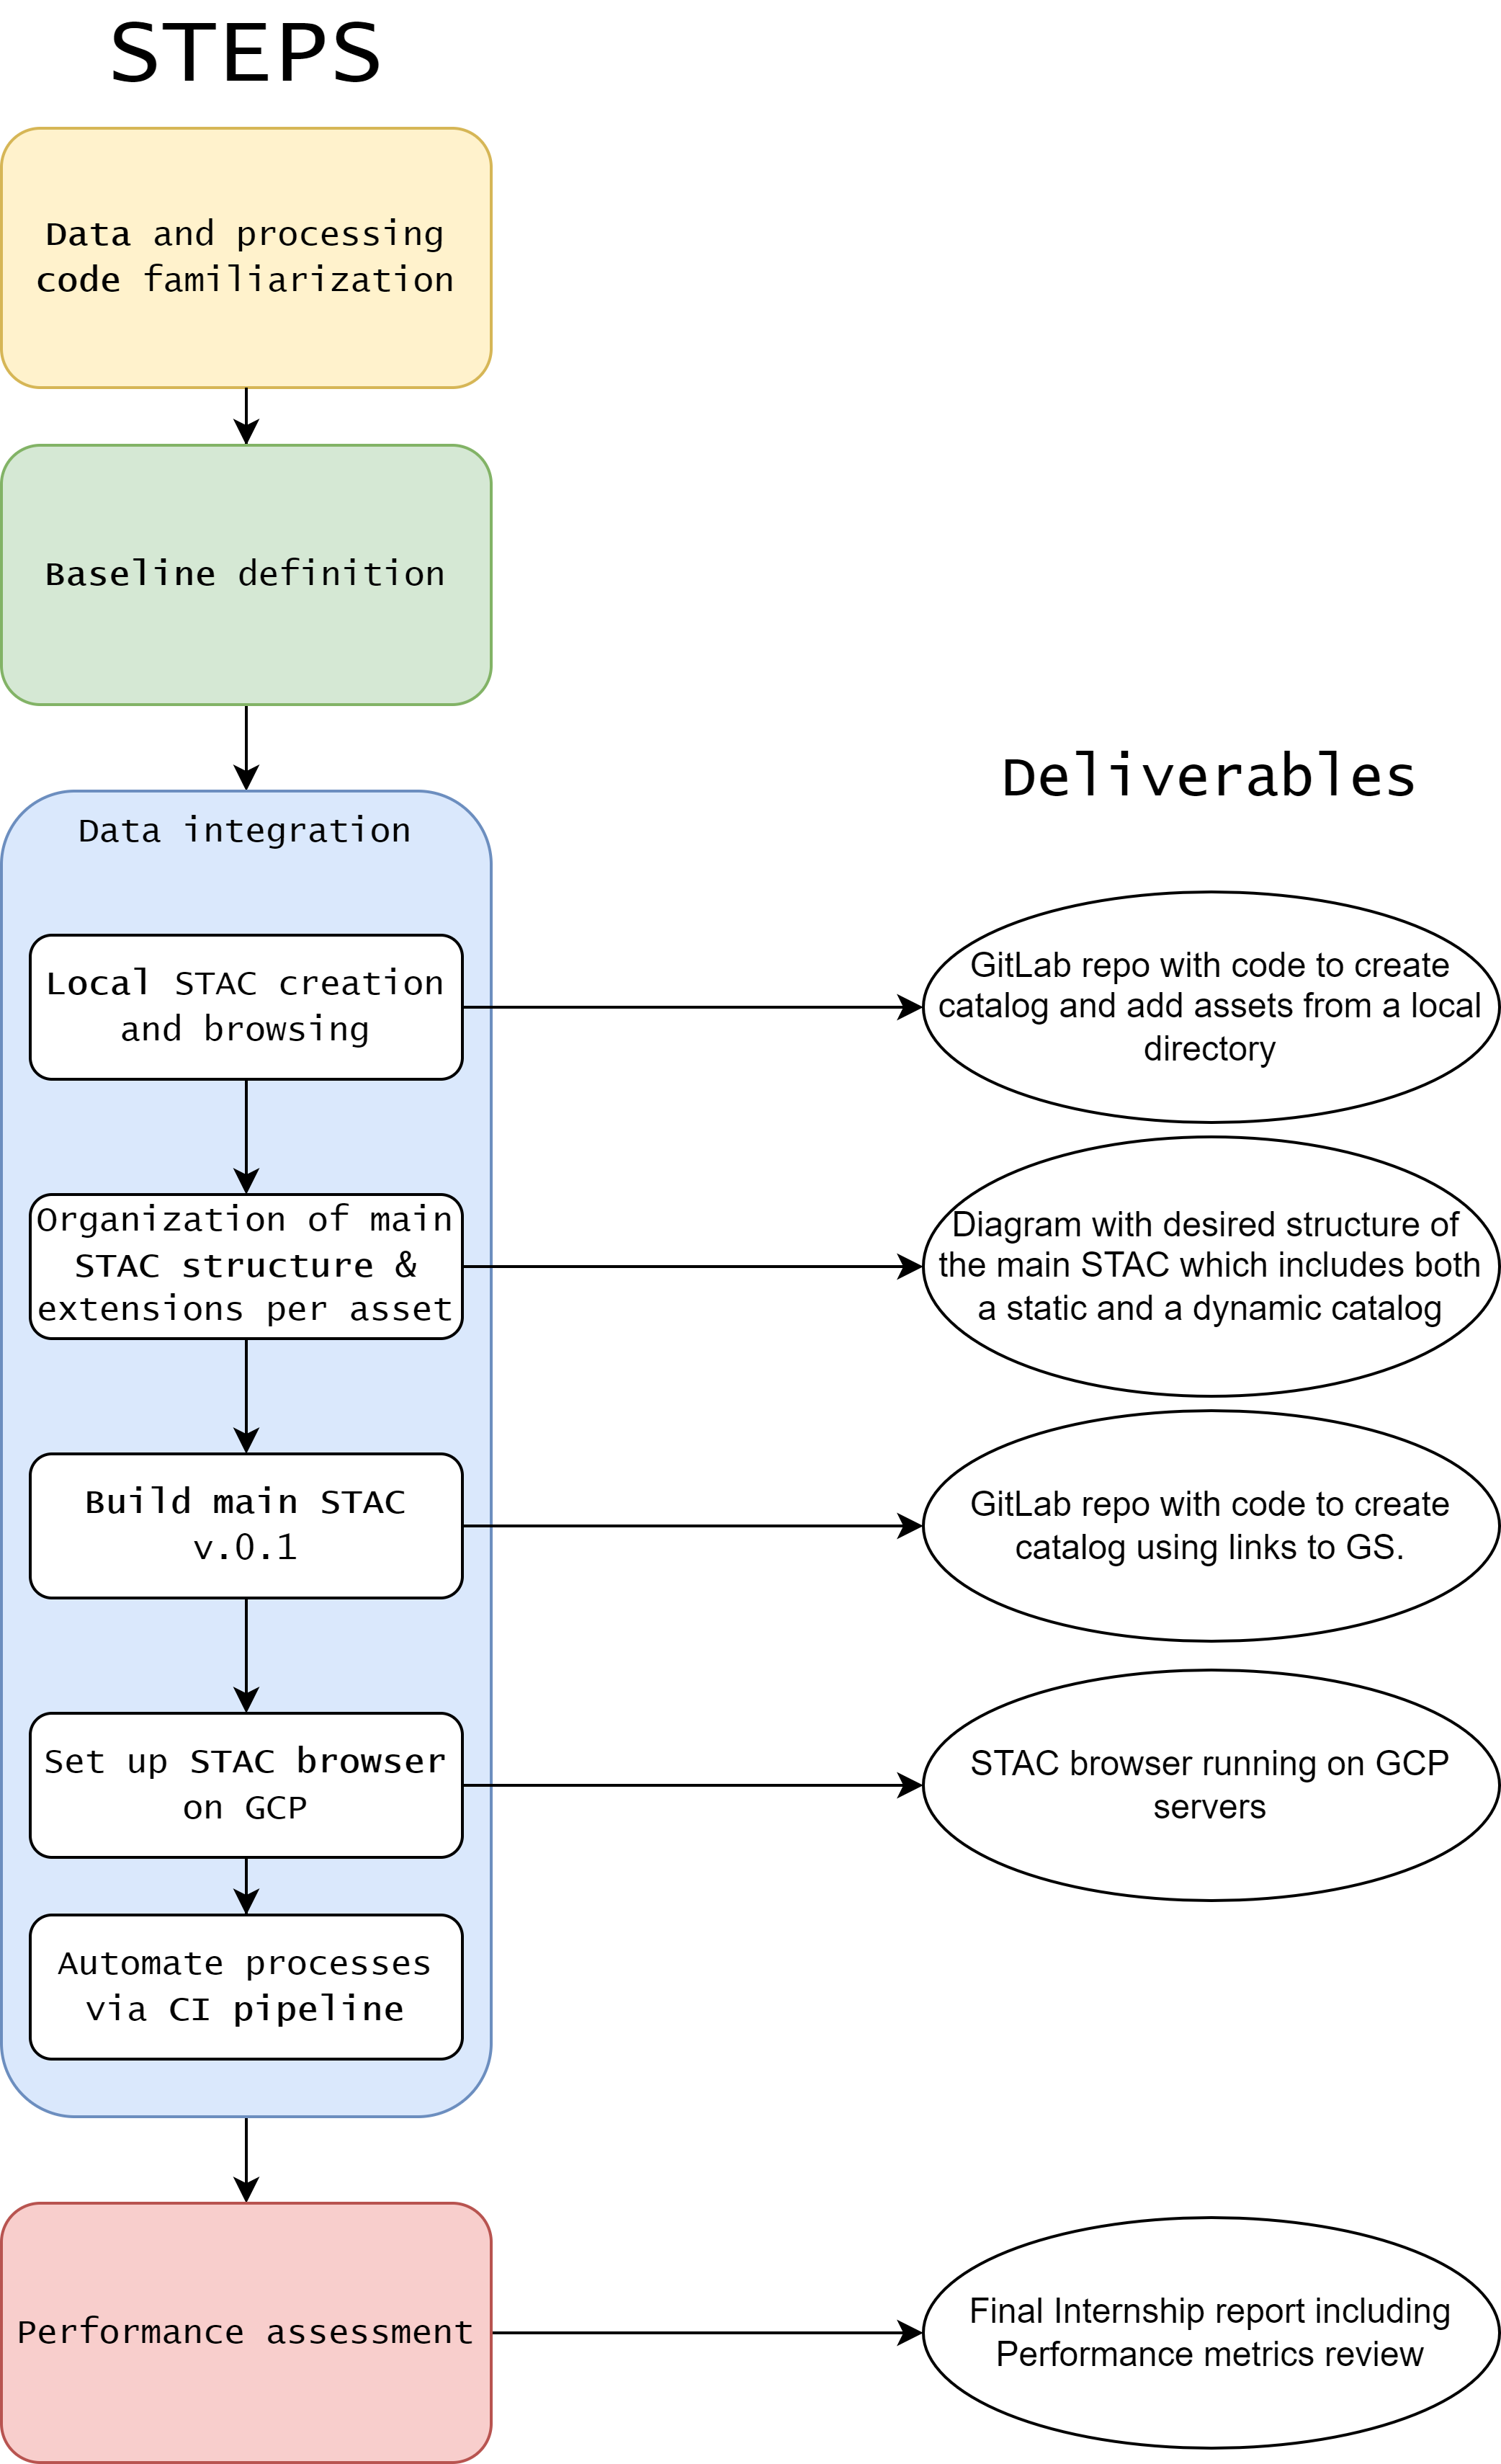
\includegraphics[width=0.6\textwidth,height=\textheight]{img/FlowChart_Internship.png}

}

\caption{\label{fig-fc}Internship flowchart}

\end{figure}%

\section{Data and processing code
familiarization}\label{data-and-processing-code-familiarization}

In this step, I will familiarize myself with the current tools used for
the processing of the images and its storage. This step will include the
understanding of cloud services and internal image processing tools and
the main datasets to be referenced on the catalog (STAC data). Moreover,
in this step an initial description of the STAC data metadata will be
performed.

\subsection{Cloud services
familiarization}\label{cloud-services-familiarization}

An overview of the cloud services used by the company will be described.
This will be mainly with the objective to understand, but not limited
to:

\begin{itemize}
\item
  Who access the data?
\item
  What are the costs of accessing it?
\item
  How often certain data is updated?
\item
  How is the data updated?
\end{itemize}

\section{Baseline scenario
definition}\label{baseline-scenario-definition}

The baseline scenario was defined as the set of methods currently being
used by members of different teams at Satelligence to find, retrieve and
visualize spatial data. This baseline scenario was evaluated
qualitatively by interviewing four members of two different teams in the
company (i.e.~The data and the operations team). To keep a balance
regarding experience of the study subjects, both the newest member of
each team and a member with at least three years in the company were
interviewed.

The questions asked during the interviews were oriented towards two main
topics that were covered during this internship: Spatial data discovery
and spatial data visualization. For both topics, the questions were
divided into questions related to raster and vector datasets. The
questions included in the interview can be found in appendix
\textbf{\#\#\#} and were meant to be open questions with multiple
possible answers.

\section{Data integration}\label{data-integration}

\subsection{Local STAC creation and
browsing}\label{local-stac-creation-and-browsing}

This step will mainly be focused on the set up of the developing
environment to both create a local STAC catalog and browse through it.
This will include:

\begin{enumerate}
\def\labelenumi{\arabic{enumi}.}
\tightlist
\item
  Creation of a virtual environment or Docker container with all the
  required packages to create a STAC catalog.
\item
  Creation of Local STAC using sample data from the company.
\item
  Browse through the STAC catalog using tools like STAC browser.
\end{enumerate}

The \textbf{deliverable} of this step will be a GitLab repository with
code to create a catalog, add assets from a local directory and browse
through them locally using STAC browser.

\subsection{Organization of main STAC structure \& extensions per
asset}\label{sec-structure}

In this step the structure of the STAC catalog will be defined. This
will involve the selection of datasets that will be referenced on the
catalog, the definition of subcatalogs and/or collections to group items
with similar metadata. An initial idea of the structure of the main STAC
catalog can be seen on Figure~\ref{fig-stac-str}. Initially, the
creation of two different subcatalogs is proposed to keep the static and
dynamic dataset separated. Moreover, the selection of the
\href{https://stac-extensions.github.io/}{STAC extensions}\footnote{STAC
  extensions are additional metadata properties that can be added to a
  dataset. (e.g.~Classes, bands, sensor-type, etc.)} used for each
dataset will be defined in this step.

\begin{figure}[H]

\centering{

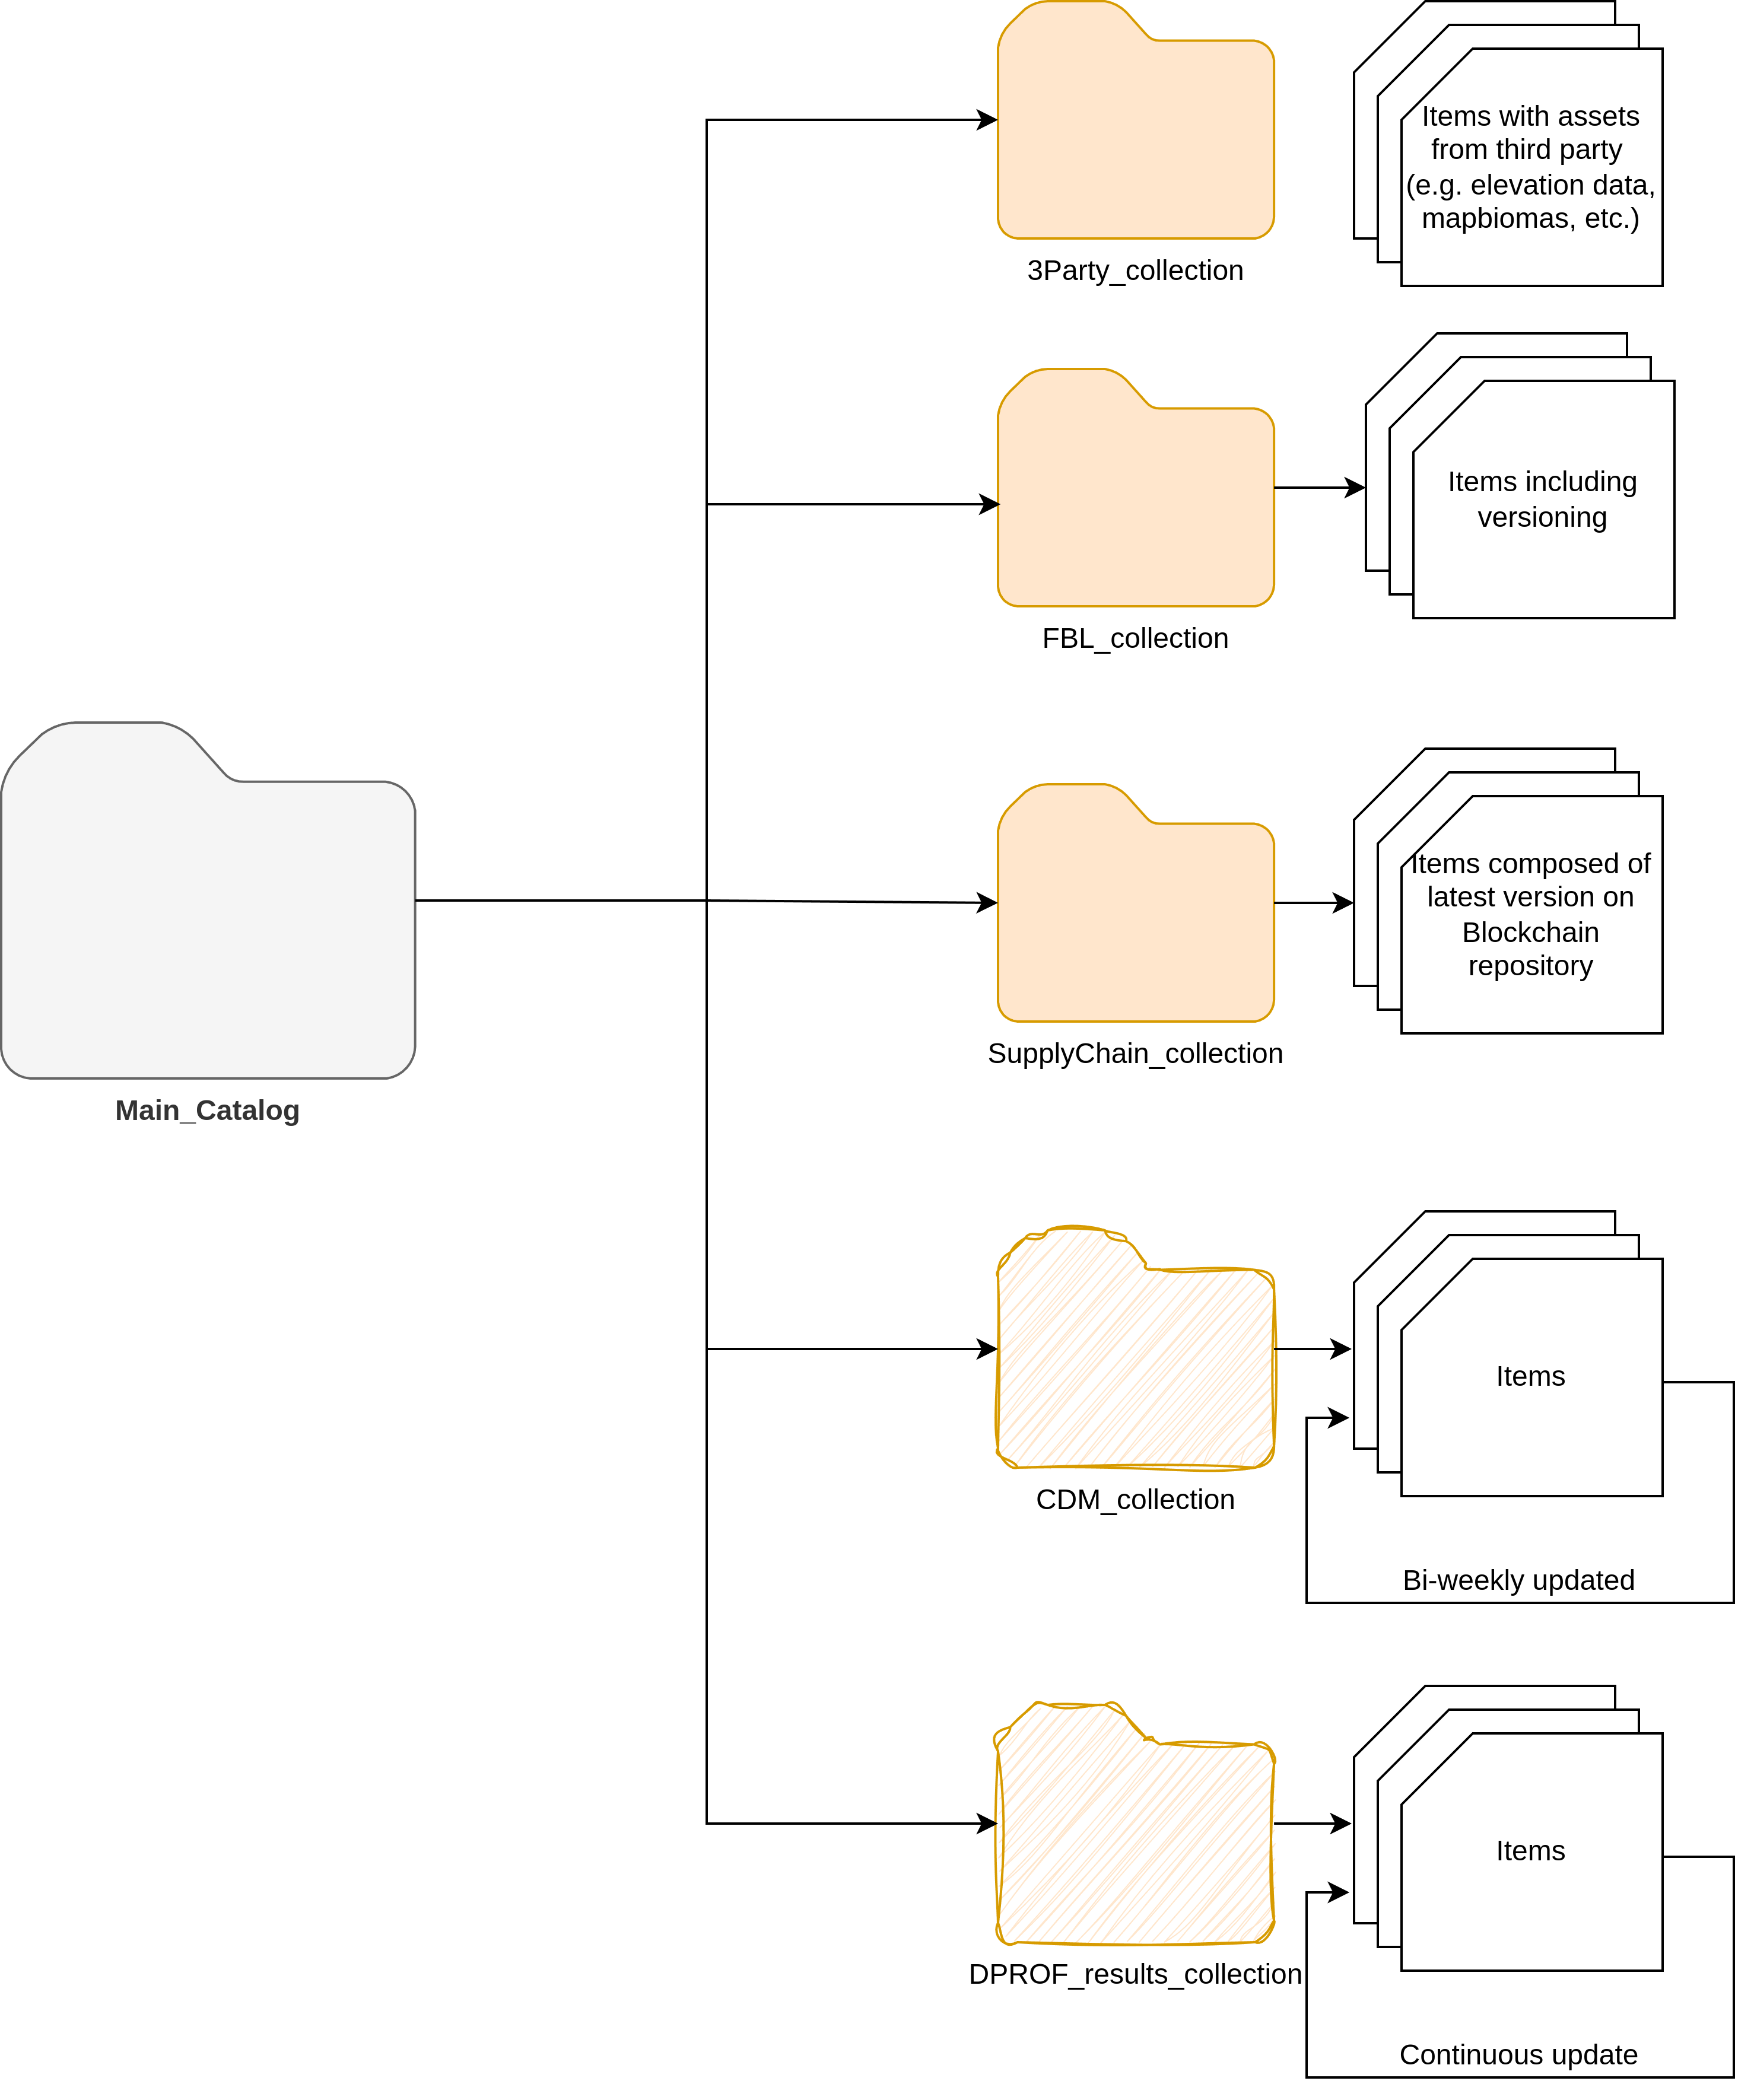
\includegraphics[width=0.9\textwidth,height=\textheight]{img/STAC_Satelligence_structure.png}

}

\caption{\label{fig-stac-str}Initial proposed STAC structure}

\end{figure}%

\subsection{Build main STAC v.0.1}\label{build-main-stac-v.0.1}

This step will focus on the building of the initial version of the main
STAC catalog, once the datasets and the overall structure has been
defined. It will involve the population of the catalog with STAC
components following the defined structure on
Section~\ref{sec-structure}. Furthermote, on this step a series of
validation tools will be used to check that the STAC catalog created is
followins the STAC spcification. These tools are part of the python
package \href{https://github.com/stac-utils/stactools}{stac-tools}.

The \textbf{deliverable} of this step will be a GitLab repository with
code to create a catalog, create collections, add assets from a
directory on the cloud and update them.

\subsection{Set up STAC browser on
GCP}\label{set-up-stac-browser-on-gcp}

In this step a version of the STAC Browser application will be deployed
using the tools from Google Cloud Platform (GCP). This application will
allow users to browse and interact with the STAC catalog through a
user-friendly interface. Additionally, this step will involve the
definition of resources and tools from GCP that will be employed to
deploy the application. For instance, the decision of doing it through a
virtual machine or on a containerized way will be made.

The \textbf{deliverable} of this step will be a the STAC browser
application running on GCP.

\subsection{Automate processes via CI
pipeline}\label{automate-processes-via-ci-pipeline}

Finally, the code to create, modify and/or deploy the STAC catalog will
be merged into a continuous integration pipeline that will allow the
integration of this catalog with other tools from the company. For
instance, the Distributed Processing Framework (DPROF), which is
satelligence's Satellite Data Processing engine.

\section{Multi-format data
visualization}\label{multi-format-data-visualization}

To assess the performance of dynamic tiling services for visualizing
Cloud Optimized GeoTIFFs (COGs) and Zarr data formats, the following
approach was undertaken. A COG containing forest baseline information
for the Riau region of Indonesia was used to create a series of Zarr
files, each representing different overviews corresponding to various
zoom levels. This preprocessing step, completed by the company prior to
the study, ensured that the same data was used across both data formats,
allowing for direct comparison.

The
\href{https://github.com/developmentseed/titiler-xarray}{TiTiler-Xarray}
service was then customized to work with the specific folder structure
of the ZARR overviews previously created. Dockerized versions of both
\href{https://github.com/developmentseed/titiler-xarray}{TiTiler-Xarray}
(for Zarr files) and
\href{https://github.com/stac-utils/titiler-pgstac}{TiTiler-PgSTAC} (for
COG files) were deployed locally.

Performance was measured by recording the response times for random tile
requests at zoom levels ranging from 9 to 18. Finally, to mitigate the
influence of cached data on response times, each iteration used a
different colormap, with a total of six colormaps employed. This
methodology enabled a systematic evaluation of the performance
differences between the two data formats in a geospatial visualization
context.

\subsection{Speed up}\label{speed-up}

The assessment of the performance of the new Data Catalog will be
measured using the baseline scenario established at the beginning of the
internship and the Speed Up metric proposed by
(\citeproc{ref-durbha_advances_2023}{Durbha et al., 2023}):

\[ SpeedUp = \frac{t_{baseline}}{t_{catalog}} \]

This metric explains how much the process to access data has sped up
thanks to the integration of cloud-based storage, the data catalog and
the browsing interface.

\chapter{Results}\label{results}

\section{Baseline scenario}\label{baseline-scenario}

\subsection{Main findings}\label{main-findings}

The main finding of the interviews were the steps followed currently to
discover, retrieve and visualize data. These steps are summarized on
Figure~\ref{fig-baseline} and show how complex and time consuming the
process of discovering and visualizing spatial data can be for a
Satelligence employee nowadays. Moreover, the steps followed were
categorized in four classes depending on how much time is generally
spent carrying out.

\begin{figure}[H]

\centering{

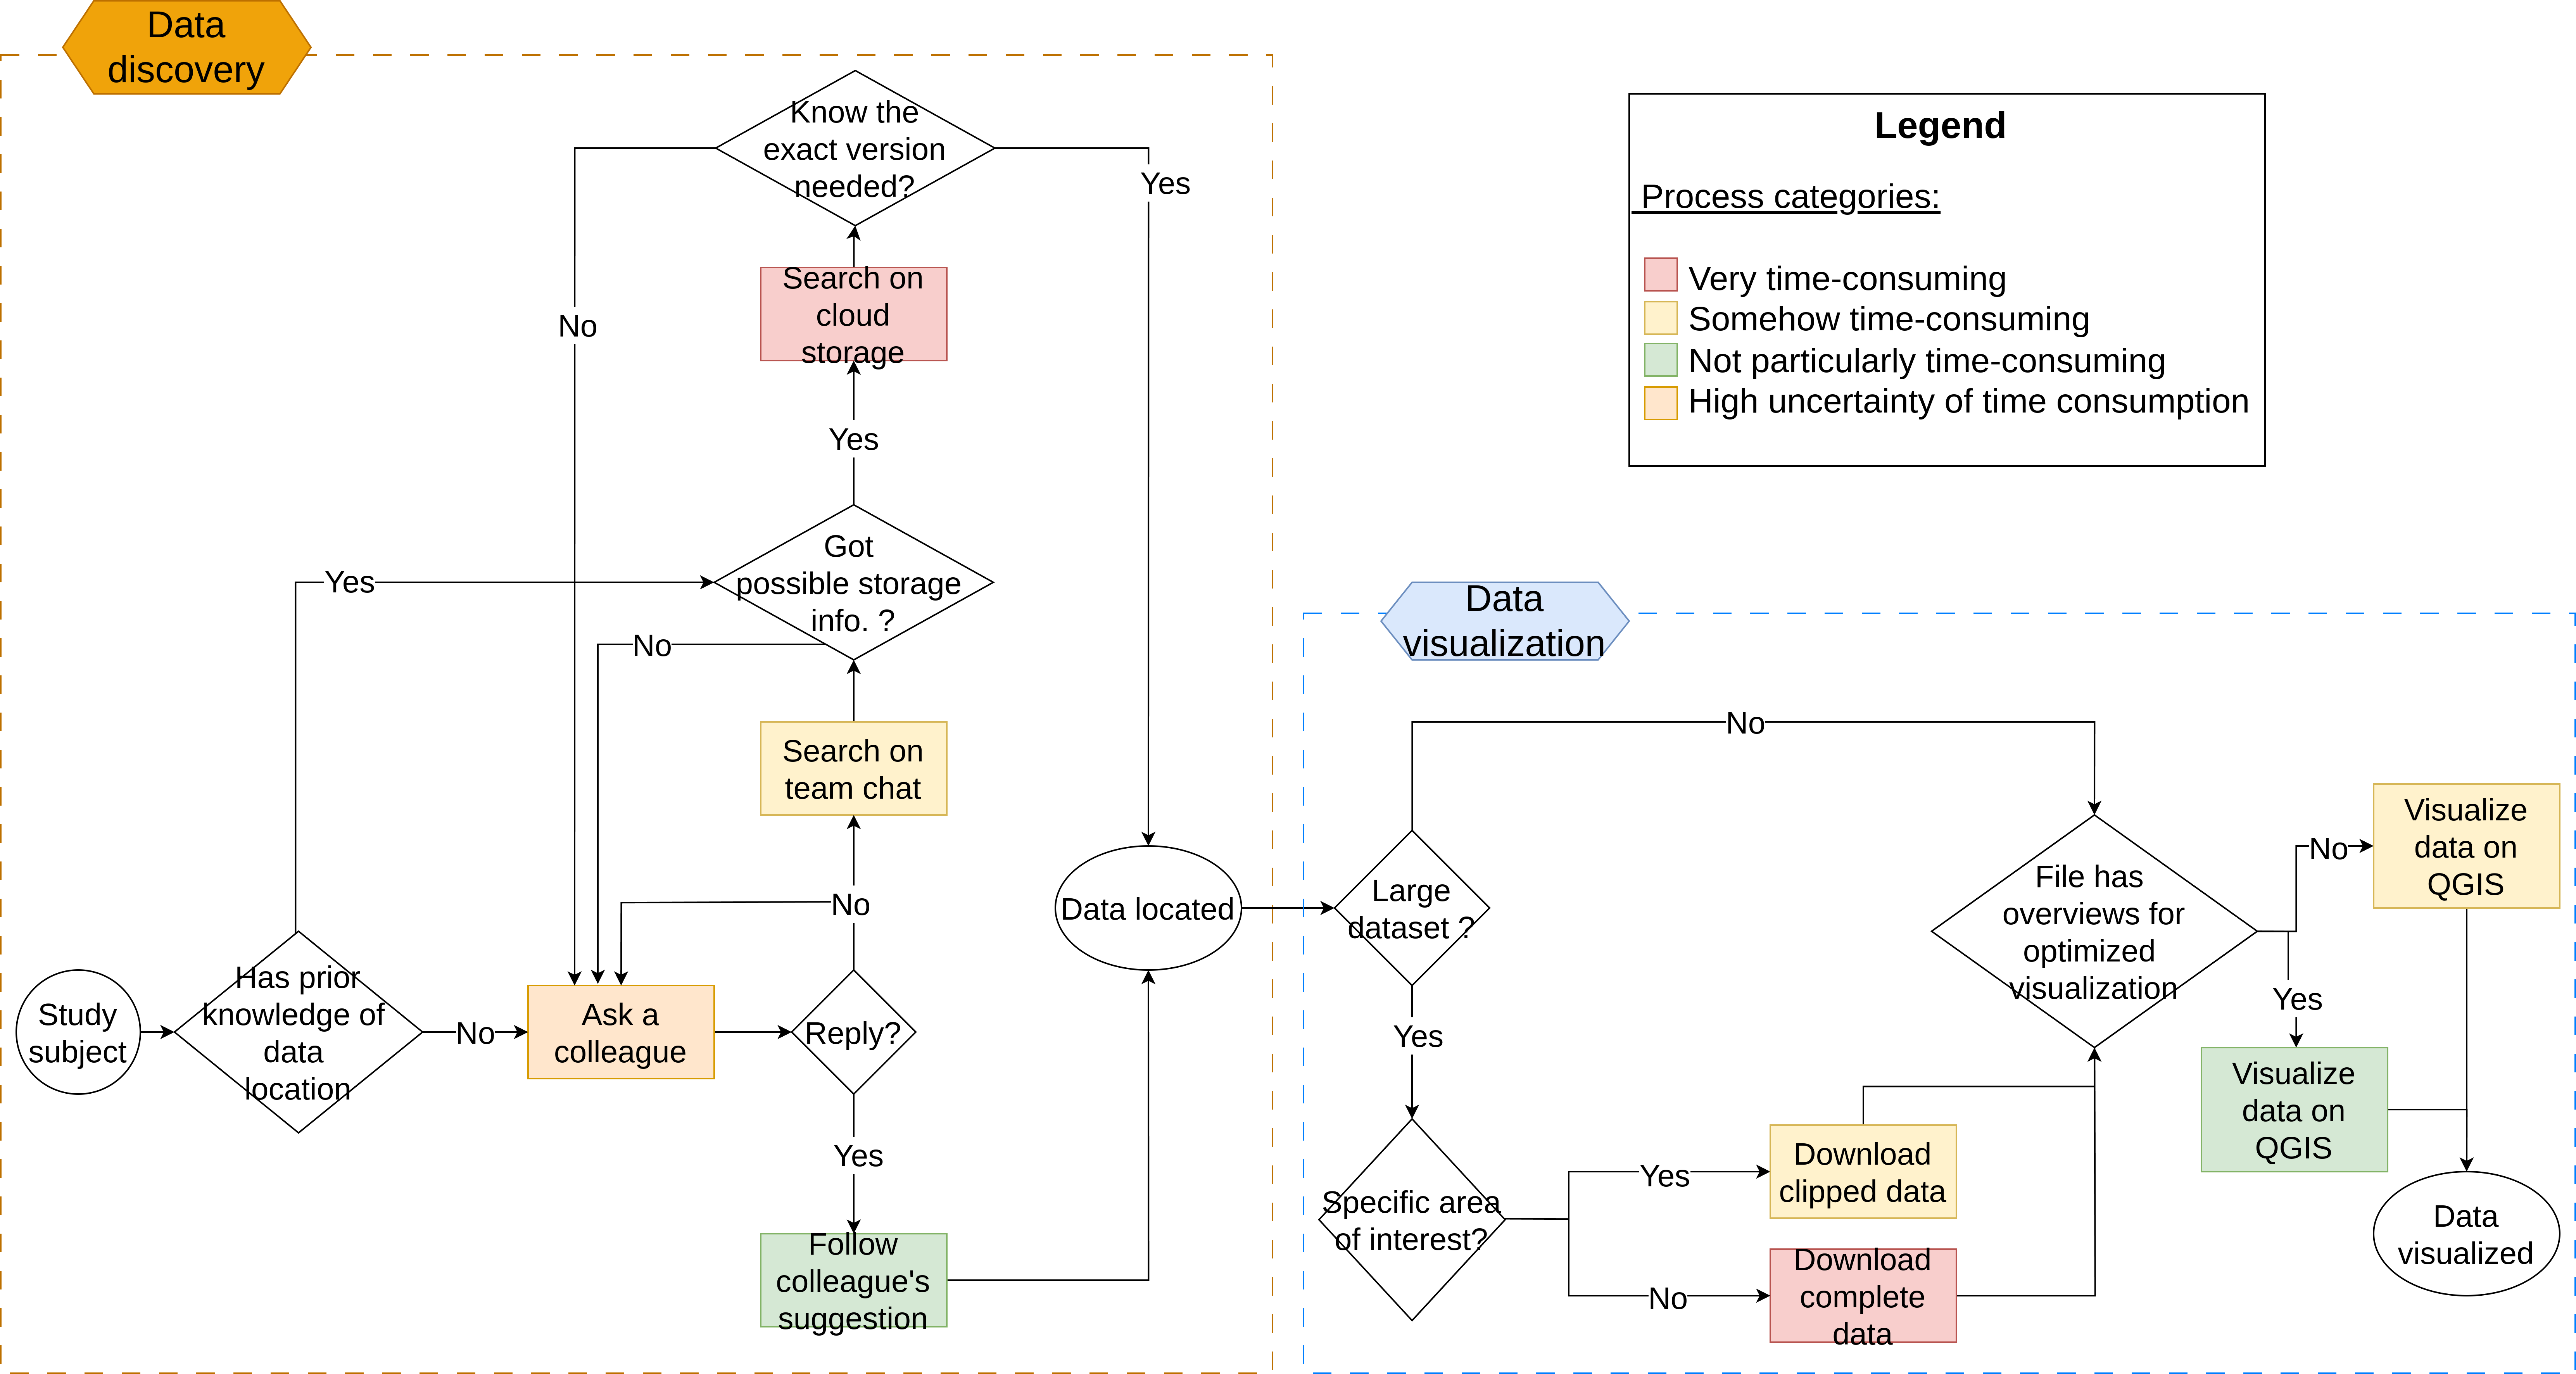
\includegraphics[width=1\textwidth,height=\textheight]{img/Baseline_data_discovery_workflow.png}

}

\caption{\label{fig-baseline}Baseline workflow}

\end{figure}%

The major pitfalls found on the process of data discovery in the company
could be summarized in:

\begin{itemize}
\tightlist
\item
  High dependency on colleagues.
\item
  Disorganized structure of Google Storage Buckets.
\item
  Experienced study subjects would find the data location faster.
\item
  Data discovery also dependent on recurrent work with a specific
  dataset (Google Console highlighted links).
\item
  Not intuitive naming of repositories.
\end{itemize}

\section{Service integration}\label{service-integration}

\emph{Explain here how eoAPI uses multiple services, how each of them
helps S11 in their data discovery and vizz tasks, and how did I manage
to deploy it}

Kubernetes

STAC-API, pgSTAC, TiTiler

\subsection{Data discovery
improvement}\label{data-discovery-improvement}

Flowchart with STAC

\section{Performance of multi-format data
visualization}\label{performance-of-multi-format-data-visualization}

TiTiler-PgSTAC \& TiTiler-xarray

\subsection{Raster formats}\label{raster-formats}

The comparison of visualization speeds with TiTiler-xarray for Zarr
datasets and TiTiler-PgSTAC for COGs are presented on
Figure~\ref{fig-format-comp}. In the figure it can be obesrved that COG
tiles are requested 2.38 times faster than the same file in ZARR format.

\begin{figure}[H]

\centering{

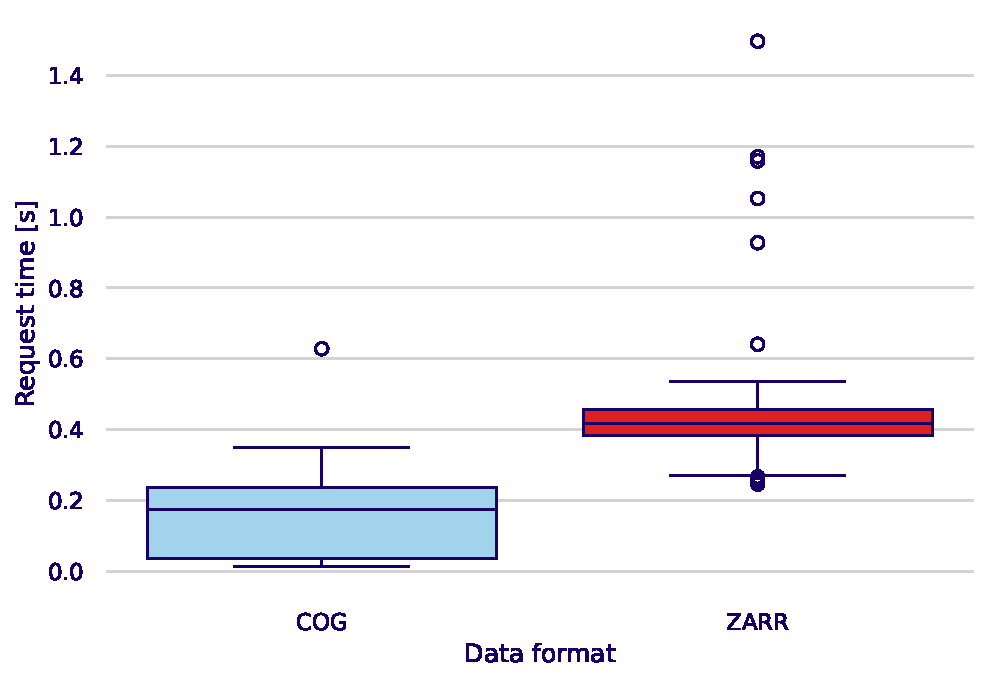
\includegraphics{FinalReport_files/figure-pdf/fig-format-comp-output-1.pdf}

}

\caption{\label{fig-format-comp}Request times depending on data format
and zoom level}

\end{figure}%

\subsection{Effects of zoom level}\label{effects-of-zoom-level}

As seen on Figure~\ref{fig-comp-zoom}, the zoom level of the map will
have an effect on the time spent requesting and getting a tile from a
tile server. In this study, it was found that the request times
decreased by a factor of -0.013 and -0.005 per zoom level for COGs and
ZARRs respectively.

\begin{figure}[H]

\centering{

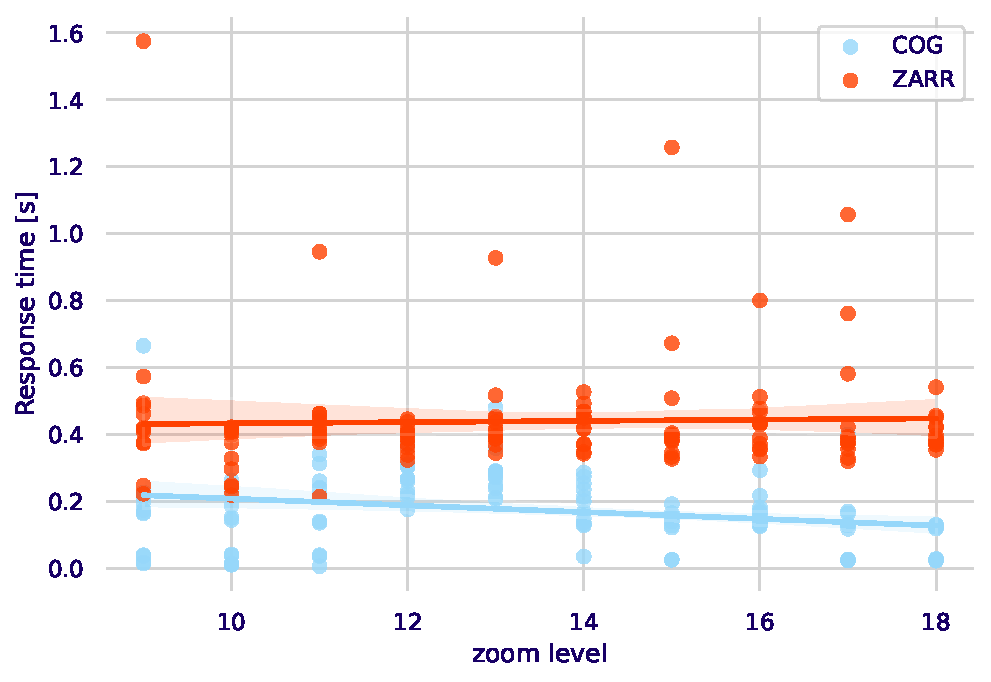
\includegraphics{FinalReport_files/figure-pdf/fig-comp-zoom-output-1.pdf}

}

\caption{\label{fig-comp-zoom}Request times depending on zoom level}

\end{figure}%

\hl{Talk about how this figure also might indicate that the way the tiles are being called by titiler xarray is not ideal?}

\chapter{Discussion}\label{discussion}

hgdcjfc rah fdxh sdfhfn dfayhgn d

gadfh

\chapter{Future work}\label{future-work}

\chapter*{References}\label{references}
\addcontentsline{toc}{chapter}{References}

\phantomsection\label{refs}
\begin{CSLReferences}{1}{0}
\bibitem[\citeproctext]{ref-brodeur_geographic_2019}
Brodeur, J., Coetzee, S., Danko, D., Garcia, S. and Hjelmager, J.
(2019). Geographic information metadata---an outlook from the
international standardization perspective. \emph{{ISPRS} International
Journal of Geo-Information}, \emph{8}(6), 280. p.
\url{https://doi.org/10.3390/ijgi8060280}

\bibitem[\citeproctext]{ref-chester_ogc_2024}
Chester, S. (2024(e)ko Januaryk 18). \emph{{OGC} forms new {GeoZarr}
standards working group to establish a zarr encoding for geospatial
data. Open geospatial consortium}.
\url{https://www.ogc.org/press-release/ogc-forms-new-geozarr-standards-working-group-to-establish-a-zarr-encoding-for-geospatial-data/}

\bibitem[\citeproctext]{ref-desruisseaux_ogc_2021}
Desruisseaux, M., Giacco, G., Goncalves, P., Manente, M. and Rouault, E.
(2021). \emph{{OGC} testbed 17: {COG}/zarr evaluation engineering
report}. \url{https://docs.ogc.org/per/21-032.html\#toc11}

\bibitem[\citeproctext]{ref-durbha_advances_2023}
Durbha, S. S., Sanyal, J., Yang, L., S Chaudhari, S., Bhangale, U.,
Bharambe, U. and Kurte, K. (2023). \emph{Advances in scalable and
intelligent geospatial analytics: Challenges and applications} (1st
ed.). {CRC} Press. \url{https://doi.org/10.1201/9781003270928}

\bibitem[\citeproctext]{ref-giri_big_2014}
Giri, K. and Lone, T. (2014). Big data -overview and challenges.
\emph{International Journal of Advanced Research in Computer Science and
Software Engineering}, \emph{4}.

\bibitem[\citeproctext]{ref-kaufmann_database_2023}
Kaufmann, M. and Meier, A. (2023). Database management. In M. Kaufmann
and A. Meier (Eds.), \emph{{SQL} and {NoSQL} databases: Modeling,
languages, security and architectures for big data management} (1--24.
pp.). Springer Nature Switzerland.
\url{https://doi.org/10.1007/978-3-031-27908-9_1}

\bibitem[\citeproctext]{ref-mishra_structured_2017}
Mishra, S. and Misra, A. (2017). Structured and unstructured big data
analytics. \emph{2017 International Conference on Current Trends in
Computer, Electrical, Electronics and Communication ({CTCEEC})},
740--746. pp. \url{https://doi.org/10.1109/CTCEEC.2017.8454999}

\bibitem[\citeproctext]{ref-ogc_ogc_2023}
OGC. (2023). \emph{{OGC} cloud optimized {GeoTIFF} standard}.
\url{https://docs.ogc.org/is/21-026/21-026.html}

\bibitem[\citeproctext]{ref-noauthor_stac-specbest-practicesmd_nodate}
RadiantEarth. (2024). \emph{Stac-spec/best-practices.md at master ·
radiantearth/stac-spec. {GitHub}}.
\url{https://github.com/radiantearth/stac-spec/blob/master/best-practices.md}

\bibitem[\citeproctext]{ref-rajabifard_spatial_2001}
Rajabifard, A. and Williamson, I. P. (2001). \emph{Spatial data
infrastructures: Concept, {SDI} hierarchy and future directions}.
\url{http://hdl.handle.net/11343/33897}

\bibitem[\citeproctext]{ref-satelligence_home_nodate}
Satelligence. (n.d.). \emph{Home - satelligence - sustainability
monitoring simplified. Satelligence}. Retrieved February 5, 2024, from
\url{https://satelligence.com/}

\bibitem[\citeproctext]{ref-satelligence_internship_2023}
Satelligence. (2023). \emph{Internship: Cataloguing and visualizing big
geodata}.

\bibitem[\citeproctext]{ref-noauthor_titiler_nodate}
\emph{{TiTiler}}. (n.d.). Retrieved February 19, 2024, from
\url{https://developmentseed.org/titiler/}

\bibitem[\citeproctext]{ref-tripathi_cloud_2020}
Tripathi, A. K., Agrawal, S. and Gupta, R. D. (2020). Cloud enabled
{SDI} architecture: A review. \emph{Earth Science Informatics},
\emph{13}(2), 211--231. pp.
\url{https://doi.org/10.1007/s12145-020-00446-9}

\bibitem[\citeproctext]{ref-zhao_scalable_2021}
Zhao, Y., Yang, X. and Vatsavai, R. R. (2021). A scalable system for
searching large-scale multi-sensor remote sensing image collections.
\emph{2021 {IEEE} International Conference on Big Data (Big Data)},
3780--3783. pp. \url{https://doi.org/10.1109/BigData52589.2021.9671679}

\end{CSLReferences}

\chapter*{Appendix}\label{appendix}
\addcontentsline{toc}{chapter}{Appendix}

\section{Code to evaluate request
times}\label{code-to-evaluate-request-times}

\begin{Shaded}
\begin{Highlighting}[]
\ImportTok{import}\NormalTok{ pandas }\ImportTok{as}\NormalTok{ pd}
\ImportTok{import}\NormalTok{ requests}
\ImportTok{import}\NormalTok{ random}

\NormalTok{tiles }\OperatorTok{=}\NormalTok{ [}\StringTok{"9/399/254"}\NormalTok{, }\StringTok{"10/800/505"}\NormalTok{, }\StringTok{"11/1603/1012"}\NormalTok{,  }\StringTok{"12/3209/2042"}\NormalTok{, }
\StringTok{"13/6407/4075"}\NormalTok{, }\StringTok{"14/12817/8159"}\NormalTok{, }\StringTok{"15/25678/16271"}\NormalTok{, }\StringTok{"16/51268/32552"}\NormalTok{, }
\StringTok{"17/102503/65134"}\NormalTok{, }\StringTok{"18/205062/130211"}\NormalTok{]}

\CommentTok{\# Tiles are slightly modified to try to avoid getting cached tiles}
\KeywordTok{def}\NormalTok{ modify\_tile(tile):}
\NormalTok{    parts }\OperatorTok{=}\NormalTok{ tile.split(}\StringTok{\textquotesingle{}/\textquotesingle{}}\NormalTok{)}
\NormalTok{    z }\OperatorTok{=} \BuiltInTok{int}\NormalTok{(parts[}\DecValTok{0}\NormalTok{])}
\NormalTok{    x }\OperatorTok{=} \BuiltInTok{int}\NormalTok{(parts[}\DecValTok{1}\NormalTok{])}
\NormalTok{    y }\OperatorTok{=} \BuiltInTok{int}\NormalTok{(parts[}\DecValTok{2}\NormalTok{])}

    \CommentTok{\# Determine the range of change based on the value of z}
    \ControlFlowTok{if}\NormalTok{ z }\OperatorTok{\textless{}=} \DecValTok{9}\NormalTok{:}
\NormalTok{        change\_range }\OperatorTok{=} \DecValTok{3}
    \ControlFlowTok{elif}\NormalTok{ z }\OperatorTok{\textless{}=} \DecValTok{12}\NormalTok{:}
\NormalTok{        change\_range }\OperatorTok{=} \DecValTok{5}
    \ControlFlowTok{elif}\NormalTok{ z }\OperatorTok{\textless{}=} \DecValTok{15}\NormalTok{:}
\NormalTok{        change\_range }\OperatorTok{=} \DecValTok{10}
    \ControlFlowTok{elif}\NormalTok{ z }\OperatorTok{\textless{}=} \DecValTok{18}\NormalTok{:}
\NormalTok{        change\_range }\OperatorTok{=} \DecValTok{50}

    \CommentTok{\# Apply the change to x and y}
\NormalTok{    x\_change }\OperatorTok{=}\NormalTok{ random.randint(}\OperatorTok{{-}}\NormalTok{change\_range, change\_range)}
\NormalTok{    y\_change }\OperatorTok{=}\NormalTok{ random.randint(}\OperatorTok{{-}}\NormalTok{change\_range, change\_range)}

\NormalTok{    new\_x }\OperatorTok{=}\NormalTok{ x }\OperatorTok{+}\NormalTok{ x\_change}
\NormalTok{    new\_y }\OperatorTok{=}\NormalTok{ y }\OperatorTok{+}\NormalTok{ y\_change}

    \CommentTok{\# Return the modified tile as a string}
    \ControlFlowTok{return} \SpecialStringTok{f"}\SpecialCharTok{\{}\NormalTok{z}\SpecialCharTok{\}}\SpecialStringTok{/}\SpecialCharTok{\{}\NormalTok{new\_x}\SpecialCharTok{\}}\SpecialStringTok{/}\SpecialCharTok{\{}\NormalTok{new\_y}\SpecialCharTok{\}}\SpecialStringTok{"}

\NormalTok{times\_zarr }\OperatorTok{=}\NormalTok{ []}
\NormalTok{times\_cog }\OperatorTok{=}\NormalTok{ []}
\NormalTok{z\_level }\OperatorTok{=}\NormalTok{ []}
\NormalTok{cmap\_picked }\OperatorTok{=}\NormalTok{ []}

\CommentTok{\# The colormaps picked can be either a customized one for S11 Forest baseline or greens\_r}
\NormalTok{cmap }\OperatorTok{=}\NormalTok{ [}\StringTok{"\_name=greens\&rescale=0,70"}\NormalTok{,}\StringTok{"\_name=greens\_r\&rescale=0,70"}\NormalTok{,}
        \StringTok{"\_name=blues\&rescale=0,90"}\NormalTok{, }\StringTok{"\_name=blues\_r\&rescale=0,90"}\NormalTok{,}
        \StringTok{"\_name=reds\&rescale=0,80"}\NormalTok{, }\StringTok{"\_name=reds\_r\&rescale=0,80"}\NormalTok{]}

\ControlFlowTok{for}\NormalTok{ i }\KeywordTok{in} \BuiltInTok{range}\NormalTok{(}\BuiltInTok{len}\NormalTok{(cmap)):}

\NormalTok{    mod\_tiles }\OperatorTok{=}\NormalTok{ [modify\_tile(tile) }\ControlFlowTok{for}\NormalTok{ tile }\KeywordTok{in}\NormalTok{ tiles]}
\NormalTok{    k }\OperatorTok{=}\NormalTok{ i}

    \ControlFlowTok{for}\NormalTok{ tile }\KeywordTok{in}\NormalTok{ mod\_tiles:}

\NormalTok{        url\_zarr }\OperatorTok{=} \SpecialStringTok{f"http://localhost:8084/tiles/WebMercatorQuad/}\SpecialCharTok{\{}\NormalTok{tile}\SpecialCharTok{\}}\SpecialStringTok{\%401x?url=gs://s11{-}tiles/zarr/separate\&variable=band\_data\&reference=false\&decode\_times=true\&consolidated=true\&colormap}\SpecialCharTok{\{}\NormalTok{cmap[k]}\SpecialCharTok{\}}\SpecialStringTok{\&return\_mask=true"}

\NormalTok{        url\_cog }\OperatorTok{=} \SpecialStringTok{f"http://localhost:8082/collections/Example\%20FBL\%20Riau/items/FBL\_V5\_2021\_Riau\_cog/tiles/WebMercatorQuad/}\SpecialCharTok{\{}\NormalTok{tile}\SpecialCharTok{\}}\SpecialStringTok{\%401x?bidx=1\&assets=data\&unscale=false\&resampling=nearest\&reproject=nearest\&colormap}\SpecialCharTok{\{}\NormalTok{cmap[k]}\SpecialCharTok{\}}\SpecialStringTok{\&return\_mask=true"}

\NormalTok{        x }\OperatorTok{=}\NormalTok{ requests.get(url\_zarr)}
\NormalTok{        times\_zarr.append(x.elapsed.total\_seconds())}

\NormalTok{        x }\OperatorTok{=}\NormalTok{ requests.get(url\_cog)}
\NormalTok{        times\_cog.append(x.elapsed.total\_seconds())}

\NormalTok{        z\_level.append(}\BuiltInTok{int}\NormalTok{(tile.split(}\StringTok{\textquotesingle{}/\textquotesingle{}}\NormalTok{)[}\DecValTok{0}\NormalTok{]))}

\NormalTok{        cmap\_picked.append(k)}

\NormalTok{data }\OperatorTok{=}\NormalTok{ pd.DataFrame([cmap\_picked, z\_level, times\_cog, times\_zarr]).T}
\NormalTok{data.columns }\OperatorTok{=}\NormalTok{ [}\StringTok{\textquotesingle{}colormap\textquotesingle{}}\NormalTok{,}\StringTok{\textquotesingle{}zoom level\textquotesingle{}}\NormalTok{,}\StringTok{\textquotesingle{}COG\textquotesingle{}}\NormalTok{, }\StringTok{\textquotesingle{}ZARR\textquotesingle{}}\NormalTok{]}

\NormalTok{data.to\_csv(}\StringTok{\textquotesingle{}request\_time\_results\_6iter.csv\textquotesingle{}}\NormalTok{)}
\end{Highlighting}
\end{Shaded}



\backmatter

\end{document}
